% !TeX root = ../thuthesis-example.tex

\chapter{对称模式挖掘算法的扩展}
本章将研究对称模式挖掘算法在复杂应用场景中的扩展。首先介绍了对称模式挖掘算法在大规模流式数据中的扩展。通过分析当前算法在流式数据中的不足之处,对区间动态规划状态进行优化,采用以空间换时间的策略提高对称模式挖掘算法在流式数据中的时间效率。然后分析了时间序列中存在多种对称模式给模式挖掘带来的困难,通过提出算法自适应的调整窗口大小,提高了对称模式挖掘的完整性。综合来看,通过调整对称模式挖掘的模型约束,可以很方便的将对称模式扩展到其他领域的应用场景。

\section{对称模式流式挖掘算法的设计与实现}
在实际场景中,经常有在对称模式发生时即时报警的应用。金融市场和股票分析是一个对数据的实时性要求很高的场景,如果在股票指数或价格时间序列出现符合某种模式的特征时能及时预报,将具有极大的应用价值。
图~\ref{fig:shanghai_point}展示了上证指数在2005年至2015年的变化时间序列,红框所示曲线符合对称模式特征。股票市场中的对称理论是一个比较小众但成熟的理论,总结为三大对称定律:其一为价格对称,即股票上涨的价格和下跌的价格相同;其二为时间对称,股票上涨持续的时间与下跌持续的时间一致;其三为高低对称,即股票上涨到一半时,后段的走势与前段的走势呈对称状。这些定律非常符合本文提出的时间序列对称模式特征。金融时间序列中的对称模式意味着当前经济周期的结束,如果能成功识别对称模式,在某种意义上则可以成功预测股票的走势,在经济周期中获得经济效益。然而,金融时间序列往往都有很强的实时性,数据是实时更新的,不具备第3节已知全局时间序列的情况。并且,金融时间序列变化快速且剧烈,因此,要求算法能快速响应。基于此,本节通过优化对称模式挖掘算法的状态推导,提高了算法的时间效率,将其扩展到了流式应用场景。
\subsection{流式对称子序列计算}
流式时间序列是一组顺序、大量、快速且连续到达的时间序列数据。
一般情况下,时间序列数据流可被视为一个随时间延续而无限增长的
动态数据集合。检测流式时间序列的对称性需要满足实时性和高效性,
即给定一个实时生成的时间序列$X=(p_1,p_2,\dots)$和时间窗口$w$,
需要在每个数据点$p_t$生成时,检测并度量时间子序列
$S=\left(p_(t-w+1),p_(t-w+2),\dots,p_t \right)$的对称性。
\begin{figure}
  \centering
  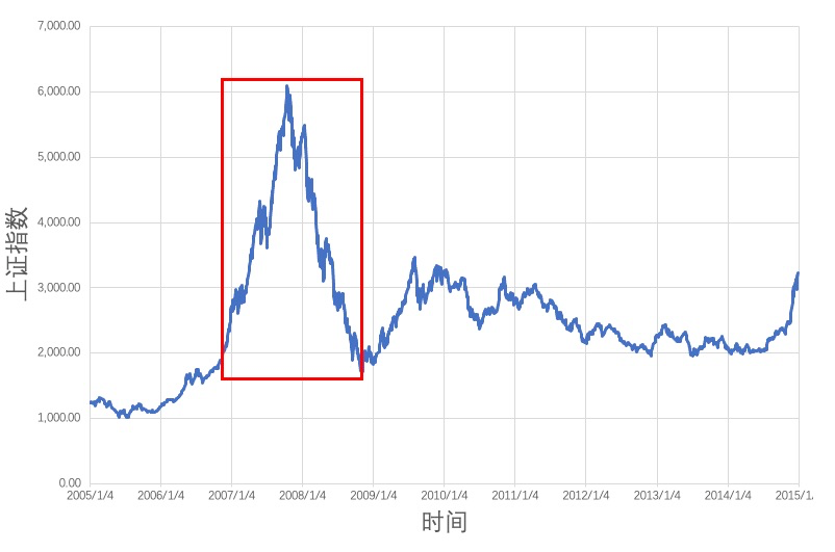
\includegraphics[width=0.86\linewidth]{shanghai_point.png}
  \caption{上证指数自2005年至2015年单日变化情况}
  \label{fig:shanghai_point}
\end{figure}
由3.1节可知,使用$DP\left(i,j\right)$表示时间序列
$Q=(p_i,p_(i+1),\dots,p_j )$的对称度。因此,
当新到来一个数据点$p_(j+1)$时,可以用公式~\ref{eq:stream_dp}
计算$DP\left(i+1,j+1\right)$。然而在该公式中,
由于$p_(j+1)$是新增点,状态$DP\left(i+2,j+1\right)$
尚未计算,不可直接使用。若直接用DTW算法计算
$S=\left(p_(t-w+1),p_(t-w+2),…,p_t \right)$
与其反转序列的DTW距离作为该序列的对称度,不仅使得对称度结果
偏高,且其时间复杂度又退化为$O\left(w^2\right)$。
因此,需要考虑如何利用已计算的状态优化流式算法。
\begin{equation}
  DP(i+1, j+1)=D(i+1, j+1)+\min \left\{\begin{array}{c}
    D P(i+2, j+1) \\
    D P(i+1, j) \\
    D P(i+2, j)
    \end{array}\right.
  \label{eq:stream_dp}
\end{equation}

图~\ref{fig:latitude_stream_matrix}展示了运煤车单次运输过程中纬度变化时间序列和
单点实时新增时对称度状态推导的变化过程,通过观察动态规划状态
的推导过程可知,当新增一个数据点$p_t$时,时间子序列
$S=\left(p_(t-w+1),p_(t-w+1),…,p_(t-1) \right)$
范围之内的对称度状态不须重新推导。因为根据3.1节介绍的时间序列
对称模式挖掘算法的数学性质,该算法满足单调性和连续性,时间序列
$S$从$p_(t-w+1)$到$p_(t-1)$之间的对称度状态$DP\left(i,j\right)$
仍然是由$DP\left(i+1,j\right)$,$DP\left(i,j-1\right)$
和$DP\left(i+1,j-1\right)$推导而来。这三个状态在对称度矩阵
中分别位于$DP\left(i,j\right)$的下方、左方和左下方。
而由图~\ref{fig:latitude_stream_matrix}的状态转移矩阵可知,
当新增数据点$p_t$时,对称度状态矩阵窗口
整体向右下方移动,并未导致$p_(t-w+1)$到$p_(t-1)$之间产生
状态失效,这就使得对称度矩阵内的状态推导顺序仍然有效。并且,
对称度模式挖掘算法的起始状态是两点间距离,也不会随着新数据点的
到来而发生改变。在推导顺序和起始状态均未改变的前提之下,只需
计算$DP\left(k,j+1\right),i+1\leq k \leq j+1$,
即图~\ref{fig:latitude_stream_matrix}所示状态转移矩阵的
最后一列状态即可。由状态转移矩阵的转移路径可知,
只需在$O\left(w\right)$的时间内便可计算出$DP\left(k,j+1\right)$,
相比通过计算原始和反转时间序列的相似性度量对称性的算法大大降低了时间复杂度。
\begin{figure}
  \centering
  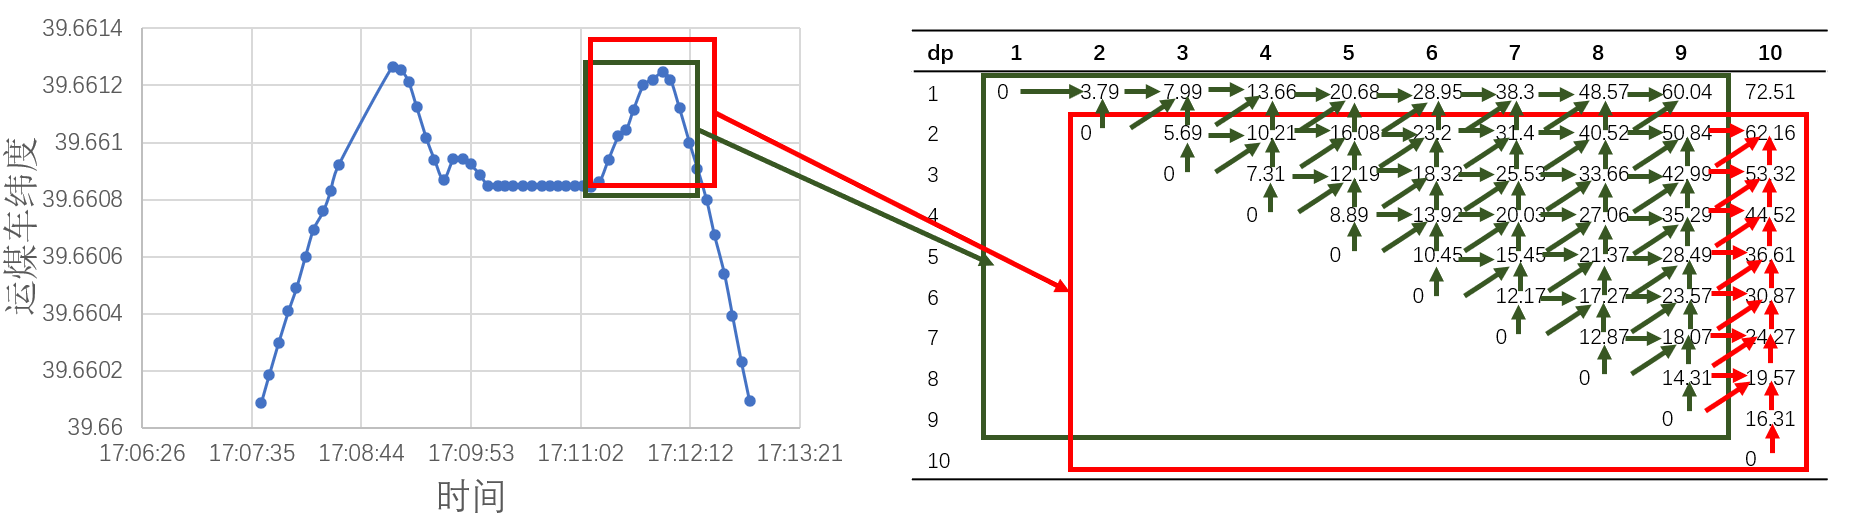
\includegraphics[width=0.86\linewidth]{latitude_stream_matrix.png}
  \caption{运煤车纬度变化与对称度状态转移过程}
  \label{fig:latitude_stream_matrix}
\end{figure}

\subsection{流式对称模式挖掘算法}
本节根据上述对称模式挖掘方法在流式数据上的分析和扩展,
提出了相应的流式挖掘算法。在流式应用场景中,
触发计算的是新数据点的到达,其他位于窗口内的数据点已经到达
并保存,无需重复输入。因此,需要自定义并维护一个双端队列,
只保存与新数据点位于同一个窗口$w$内的数据点,作为流式计算的
状态信息。并且,由图~\ref{fig:latitude_stream_matrix}的
状态转移矩阵可以发现,对称模式流式挖掘算法模型并不需要保存
完整的对称度矩阵,当新增一个数据点$p_t$时,只需要用到
对称度矩阵的最后一列状态来推导和$p_t$相关的状态,从而优化
空间复杂度。总之,对称模式流式挖掘算法只需要长度约束$w$和
新增数据点$p_t$作为输入,此外,由于流式数据是动态、源源不断
到来的,模式识别需要实时报警,且允许出现存在重叠的对称模式。
因此,之前计算对称模式第二类阈值的方法不再适用,只使用第一类
阈值过滤对称模式。算法4.1展示了时间序列对称模式流式挖掘算法
的计算流程,第1-4行对流式框架所需的时间序列$X$和对称度阈值$d$,
第5-12行进行冷启动处理,当数据点数小于$w$时更新对称度状态$dp$
并统一判断为非对称模式。第13-17行倒序计算流式时间序列的对称性,
以保证下次处理时$X$也只有$w$个数据点,
第18行将时间序列$X$中第一个数据点删除,第19-23行
对数据点数大于$w$的时间序列计算对称度状态,
并通过比较是否超过对称度阈值,判断是否为对称模式。
该算法的时间和空间复杂度
均为$O\left(w\right)$,具有较高的时间效率和较快的响应速度。

\renewcommand{\algorithmicrequire}{\textbf{输入:}\unskip}
\renewcommand{\algorithmicensure}{\textbf{输出:}\unskip}

\begin{algorithm}
  \caption{时间序列对称模式流式挖掘算法$calculate\_streaming\_symmtric\_pattern$}
  \label{alg:streaming_symmetric_pattern}
  \small
  \begin{algorithmic}
    \REQUIRE 新数据点$p_t$,长度约束$w$
    \ENSURE 布尔型变量,标志$S=\left(p_(t-w+1),p_(t-w+2),…,p_t \right)$是否为对称子序列

    \STATE 将$p_t$置于时间序列$X$中
    \IF{$t > 1$}
      \STATE $d=d+D\left(p_{t}, p_{t-1}\right)$
    \ENDIF

    \IF{$t < w$}
      \STATE $i \leftarrow t-1$
      \WHILE{$i > 1$}
        \STATE $dp_{i,t} \leftarrow D\left(p_{i}, p_{t} \right) + \min \left(dp_{i,t-1},dp_{i+1,t},dp_{i+1,t-1}\right)$
        \STATE $i \leftarrow i-1$
      \ENDWHILE
      \RETURN false
    \ENDIF

    \STATE $i \leftarrow t-1$
    \WHILE{$i > t-w+1$}
      \STATE $dp_{i,t} \leftarrow D\left(p_{i}, p_{t} \right) + \min \left(dp_{i,t-1},dp_{i+1,t},dp_{i+1,t-1}\right)$
      \STATE $i \leftarrow i-1$
    \ENDWHILE

    \STATE 将$p_(t-w+1)$时间序列X中删除;
    \IF{$dp_{t-w+1,t}/t > d/(n-1)$}
      \RETURN false
    \ELSE
      \RETURN true
    \ENDIF
  \end{algorithmic}
\end{algorithm}

\section{自适应窗口的设计与实现}
时间序列的数据和模式均具有很强的随机性,同一个时间序列中的
对称模式其数据点个数可能不严格相等,而是处于某个合理范围之内。
以挖掘机为例,挖掘不同的坑道时,斗杆移动的轨迹就不同。
人为设置时间序列对称模式的长度尽管可以挖掘出所有的对称模式,
但是每个模式的信息却经常存在缺失,
图~\ref{fig:excavator_diff_route}展示了挖掘机在不同坑道
挖掘作业斗杆外摆工况变化时间序列。若设定对称子序列的数据点个数
即窗口长度为坑道a的序列长度,则坑道b的对称子序列不能完全挖掘。
除此之外,一个时间窗口往往只能挖掘出固定的一种对称模式,
挖掘多个模式就需要不同长度的时间窗口。因此,当需要挖掘的
对称模式长度不一时,窗口需要自适应的变化。为避免引入新的参数,
本节利用数据点差分的分布特征,使得窗口能自动调节大小。
\begin{figure}
  \centering
  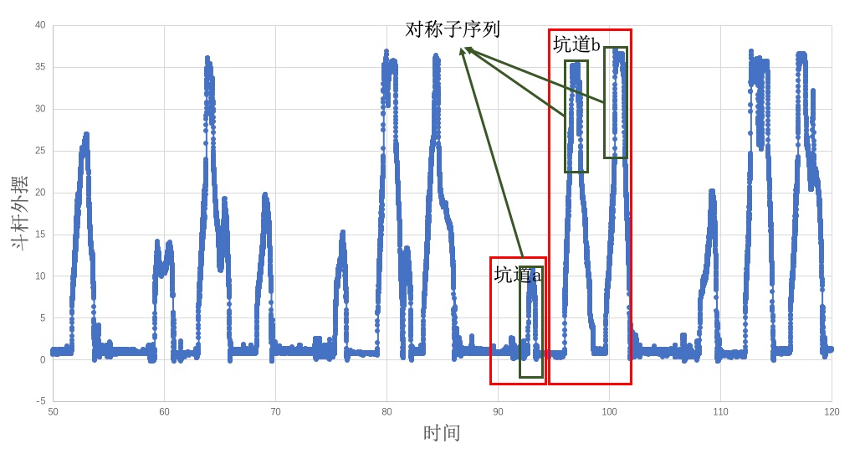
\includegraphics[width=0.86\linewidth]{excavator_diff_route.png}
  \caption{挖掘机在不同坑道挖掘作业斗杆外摆工况时间序列}
  \label{fig:excavator_diff_route}
\end{figure}

根据时间序列对称性的定义,在设定对称子序列的最小长度$w$之后,
对称时间序列$X=\left(p_1,p_2,…,p_n \right)$的首尾点
$p_1$和$p_n$必定匹配。换言之,首尾点的距离若接近0,
则证明该窗口大小合适;若远大于0,则证明需调大窗口,
以完整获取对称子序列的全部信息。
因此,可以使用时间子序列首尾点的距离来衡量窗口大小设置得
是否合适。

然而,真实工业场景中的匹配数据点往往具有误差,
并不一定满足首尾点距离为0。因此,本文考虑利用相邻点距离
所组成数据集的分布特点,判断窗口是否应当扩张。
根据工业大数据时间序列点的随机性,首尾数据点的距离所组成的
数据集应满足正态分布的特点[13],且其均值为0。也就是说,
若一个窗口内的相邻点距离集合为
$s=\left\{D\left(p_{1}, p_{2}\right), D\left(p_{2}, p_{3}\right), \ldots, D\left(p_{n-1}, p_{n}\right)\right\}$,
则首尾数据点距离的应满足均值为$\mu=0$且标准差$\sigma=\sigma_s$
的正态分布。按照3$\sigma$原则,首尾数据点的距离应在
$\left[0,3\sigma\right]$范围之内。

\renewcommand{\algorithmicrequire}{\textbf{输入:}\unskip}
\renewcommand{\algorithmicensure}{\textbf{输出:}\unskip}

\begin{algorithm}
  \caption{自适应窗口算法$adaptive\_window$}
  \label{alg:adaptive_window}
  \small
  \begin{algorithmic}
    \REQUIRE 时间序列$X=\left(p_1,p_2,…,p_n\right)$,长度约束$w$
    \ENSURE 调整后的窗口大小$t$

    \STATE $\sigma=\operatorname{mad}(X, w)$
    \STATE $t \leftarrow w$
    \STATE $i \leftarrow 1$
    \WHILE{$i+t<|X| \& \& t<2 \times w \& \& D\left(p_{i}, p_{i+1}\right)>3 \sigma$}
      \STATE $t \leftarrow t+1$
    \ENDWHILE
    \RETURN $t$
  \end{algorithmic}
\end{algorithm}

此外,考虑到数据集为相邻点的距离,属于差分计算。
因此,相比标准差,绝对中位差更加符合数据集的特点。
绝对中位差指的是所有元素与其中位数的偏差的绝对值,
其度量数据集合中的零散程度,相比标准差具有更强的鲁棒性,
且已有较为成熟的近似算法加快计算[14]。因此,本节使用窗口内
相邻数据点的距离绝对中位差作为$\sigma$,
首尾点的距离应在$\left[0,3\sigma\right]$之间。
指定窗口的最小时长约束$w$,若窗口的最终点和起始点的距离
在$\left[0,3\sigma\right]$范围之内,则窗口闭合。
否则,则继续调大窗口,直到窗口大小为$2w$为止。
因为若窗口大小超出$2w$,则挖掘出的对称子序列可能覆盖多个
不重叠对称子序列,使得最终结果不精确。具体的计算流程如算法~\ref{alg:adaptive_window}所示。

\section{本章小结}
本章主要介绍了时间序列对称模式挖掘在更多应用场景下的扩展。
首先,流式时间序列数据作为一种在工业和金融领域经常出现的数据
类型,对其进行对称模式挖掘具有重要的研究价值。但是,
度量所有时间子序列的对称性会产生大量重复计算,时间效率低,
且对称度阈值也不好判定。本章根据全局时间序列对称模式挖掘算法
的状态推导方式,在对称度矩阵上创造性地引入了滑动窗口,
在不违反对称度状态连续性和单调性的前提下,采用以空间换时间的
策略将流式对称模式的计算时间复杂度由$O\left(w^2\right)$
提升至了$O\left(w\right)$。
此外,为了在时间序列中挖掘完整的对称模式,本章还在对称模式的
挖掘过程中引入了自适应窗口,通过时间序列的数据特征自动地调节
窗口大小,以保证挖掘对称模式的完整性。对称模式挖掘在不同的
应用中具有很好的可扩展性,通过约定不同的约束可以灵活地调整
对称模式挖掘算法,从而满足不同场景的需要。

% 模板支持 BibTeX 和 BibLaTeX 两种方式处理参考文献。
% 下文主要介绍 BibTeX 配合 \pkg{natbib} 宏包的主要使用方法。


% \section{顺序编码制}

% 在顺序编码制下,默认的 \cs{cite} 命令同 \cs{citep} 一样,序号置于方括号中,
% 引文页码会放在括号外。
% 统一处引用的连续序号会自动用短横线连接。

% \thusetup{
%   cite-style = super,
% }
% \begin{tabular}{l@{\quad$\Rightarrow$\quad}l}
%   \verb|\cite{zhangkun1994}|               & \cite{zhangkun1994}               \\
%   \verb|\citet{zhangkun1994}|              & \citet{zhangkun1994}              \\
%   \verb|\citep{zhangkun1994}|              & \citep{zhangkun1994}              \\
%   \verb|\cite[42]{zhangkun1994}|           & \cite[42]{zhangkun1994}           \\
%   \verb|\cite{zhangkun1994,zhukezhen1973}| & \cite{zhangkun1994,zhukezhen1973} \\
% \end{tabular}


% 也可以取消上标格式,将数字序号作为文字的一部分。
% 建议全文统一使用相同的格式。

% \thusetup{
%   cite-style = inline,
% }
% \begin{tabular}{l@{\quad$\Rightarrow$\quad}l}
%   \verb|\cite{zhangkun1994}|               & \cite{zhangkun1994}               \\
%   \verb|\citet{zhangkun1994}|              & \citet{zhangkun1994}              \\
%   \verb|\citep{zhangkun1994}|              & \citep{zhangkun1994}              \\
%   \verb|\cite[42]{zhangkun1994}|           & \cite[42]{zhangkun1994}           \\
%   \verb|\cite{zhangkun1994,zhukezhen1973}| & \cite{zhangkun1994,zhukezhen1973} \\
% \end{tabular}



% \section{著者-出版年制}

% 著者-出版年制下的 \cs{cite} 跟 \cs{citet} 一样。

% \thusetup{
%   cite-style = author-year,
% }
% \begin{tabular}{l@{\space$\Rightarrow$\space}l}
%   \verb|\cite{zhangkun1994}|                & \cite{zhangkun1994}                \\
%   \verb|\citet{zhangkun1994}|               & \citet{zhangkun1994}               \\
%   \verb|\citep{zhangkun1994}|               & \citep{zhangkun1994}               \\
%   \verb|\cite[42]{zhangkun1994}|            & \cite[42]{zhangkun1994}            \\
%   \verb|\citep{zhangkun1994,zhukezhen1973}| & \citep{zhangkun1994,zhukezhen1973} \\
% \end{tabular}

% \vskip 2ex
% \thusetup{
%   cite-style = super,
% }
% 注意,引文参考文献的每条都要在正文中标注
% \cite{zhangkun1994,zhukezhen1973,dupont1974bone,zhengkaiqing1987,%
%   jiangxizhou1980,jianduju1994,merkt1995rotational,mellinger1996laser,%
%   bixon1996dynamics,mahui1995,carlson1981two,taylor1983scanning,%
%   taylor1981study,shimizu1983laser,atkinson1982experimental,%
%   kusch1975perturbations,guangxi1993,huosini1989guwu,wangfuzhi1865songlun,%
%   zhaoyaodong1998xinshidai,biaozhunhua2002tushu,chubanzhuanye2004,%
%   who1970factors,peebles2001probability,baishunong1998zhiwu,%
%   weinstein1974pathogenic,hanjiren1985lun,dizhi1936dizhi,%
%   tushuguan1957tushuguanxue,aaas1883science,fugang2000fengsha,%
%   xiaoyu2001chubanye,oclc2000about,scitor2000project%
% }。
